\section{Projeção do grafo de conhecimento}

A base foi ampliada com uma projeção de grafo de propriedades destinada a perguntas estruturais e agregadas que não devem ser respondidas pela recuperação de poucos fragmentos. Essa camada complementa a busca semântica: perguntas sobre o conteúdo dos trabalhos continuam sendo encaminhadas ao RAG vetorial, enquanto contagens e relações explícitas podem ser obtidas por consultas determinísticas. Nesta etapa, o grafo foi persistido no próprio PostgreSQL para manter metadados, vetores, nós, arestas e proveniência sob as mesmas transações e restrições de integridade, sem introduzir um segundo servidor.

Foram definidos quatro tipos de nó: \texttt{work}, para o trabalho identificado pelo SHA-256 do PDF; \texttt{person}, para participante principal ou orientador; \texttt{edition}, para as edições 1 a 5; e \texttt{course}, para o curso informado no cabeçalho. As arestas partem do trabalho e utilizam os tipos \texttt{AUTHORED\_BY}, \texttt{ADVISED\_BY}, \texttt{PRESENTED\_IN} e \texttt{ASSOCIATED\_WITH\_COURSE}. Cada aresta conserva o documento e a página de origem, de modo que uma relação possa ser rastreada até o PDF que a sustenta.

\begin{figure}[!htbp]
\centering
\begin{minipage}{\linewidth}
\caption{Modelo entidade-relacionamento da projeção do grafo de conhecimento}
\label{fig:der-grafo-conhecimento}
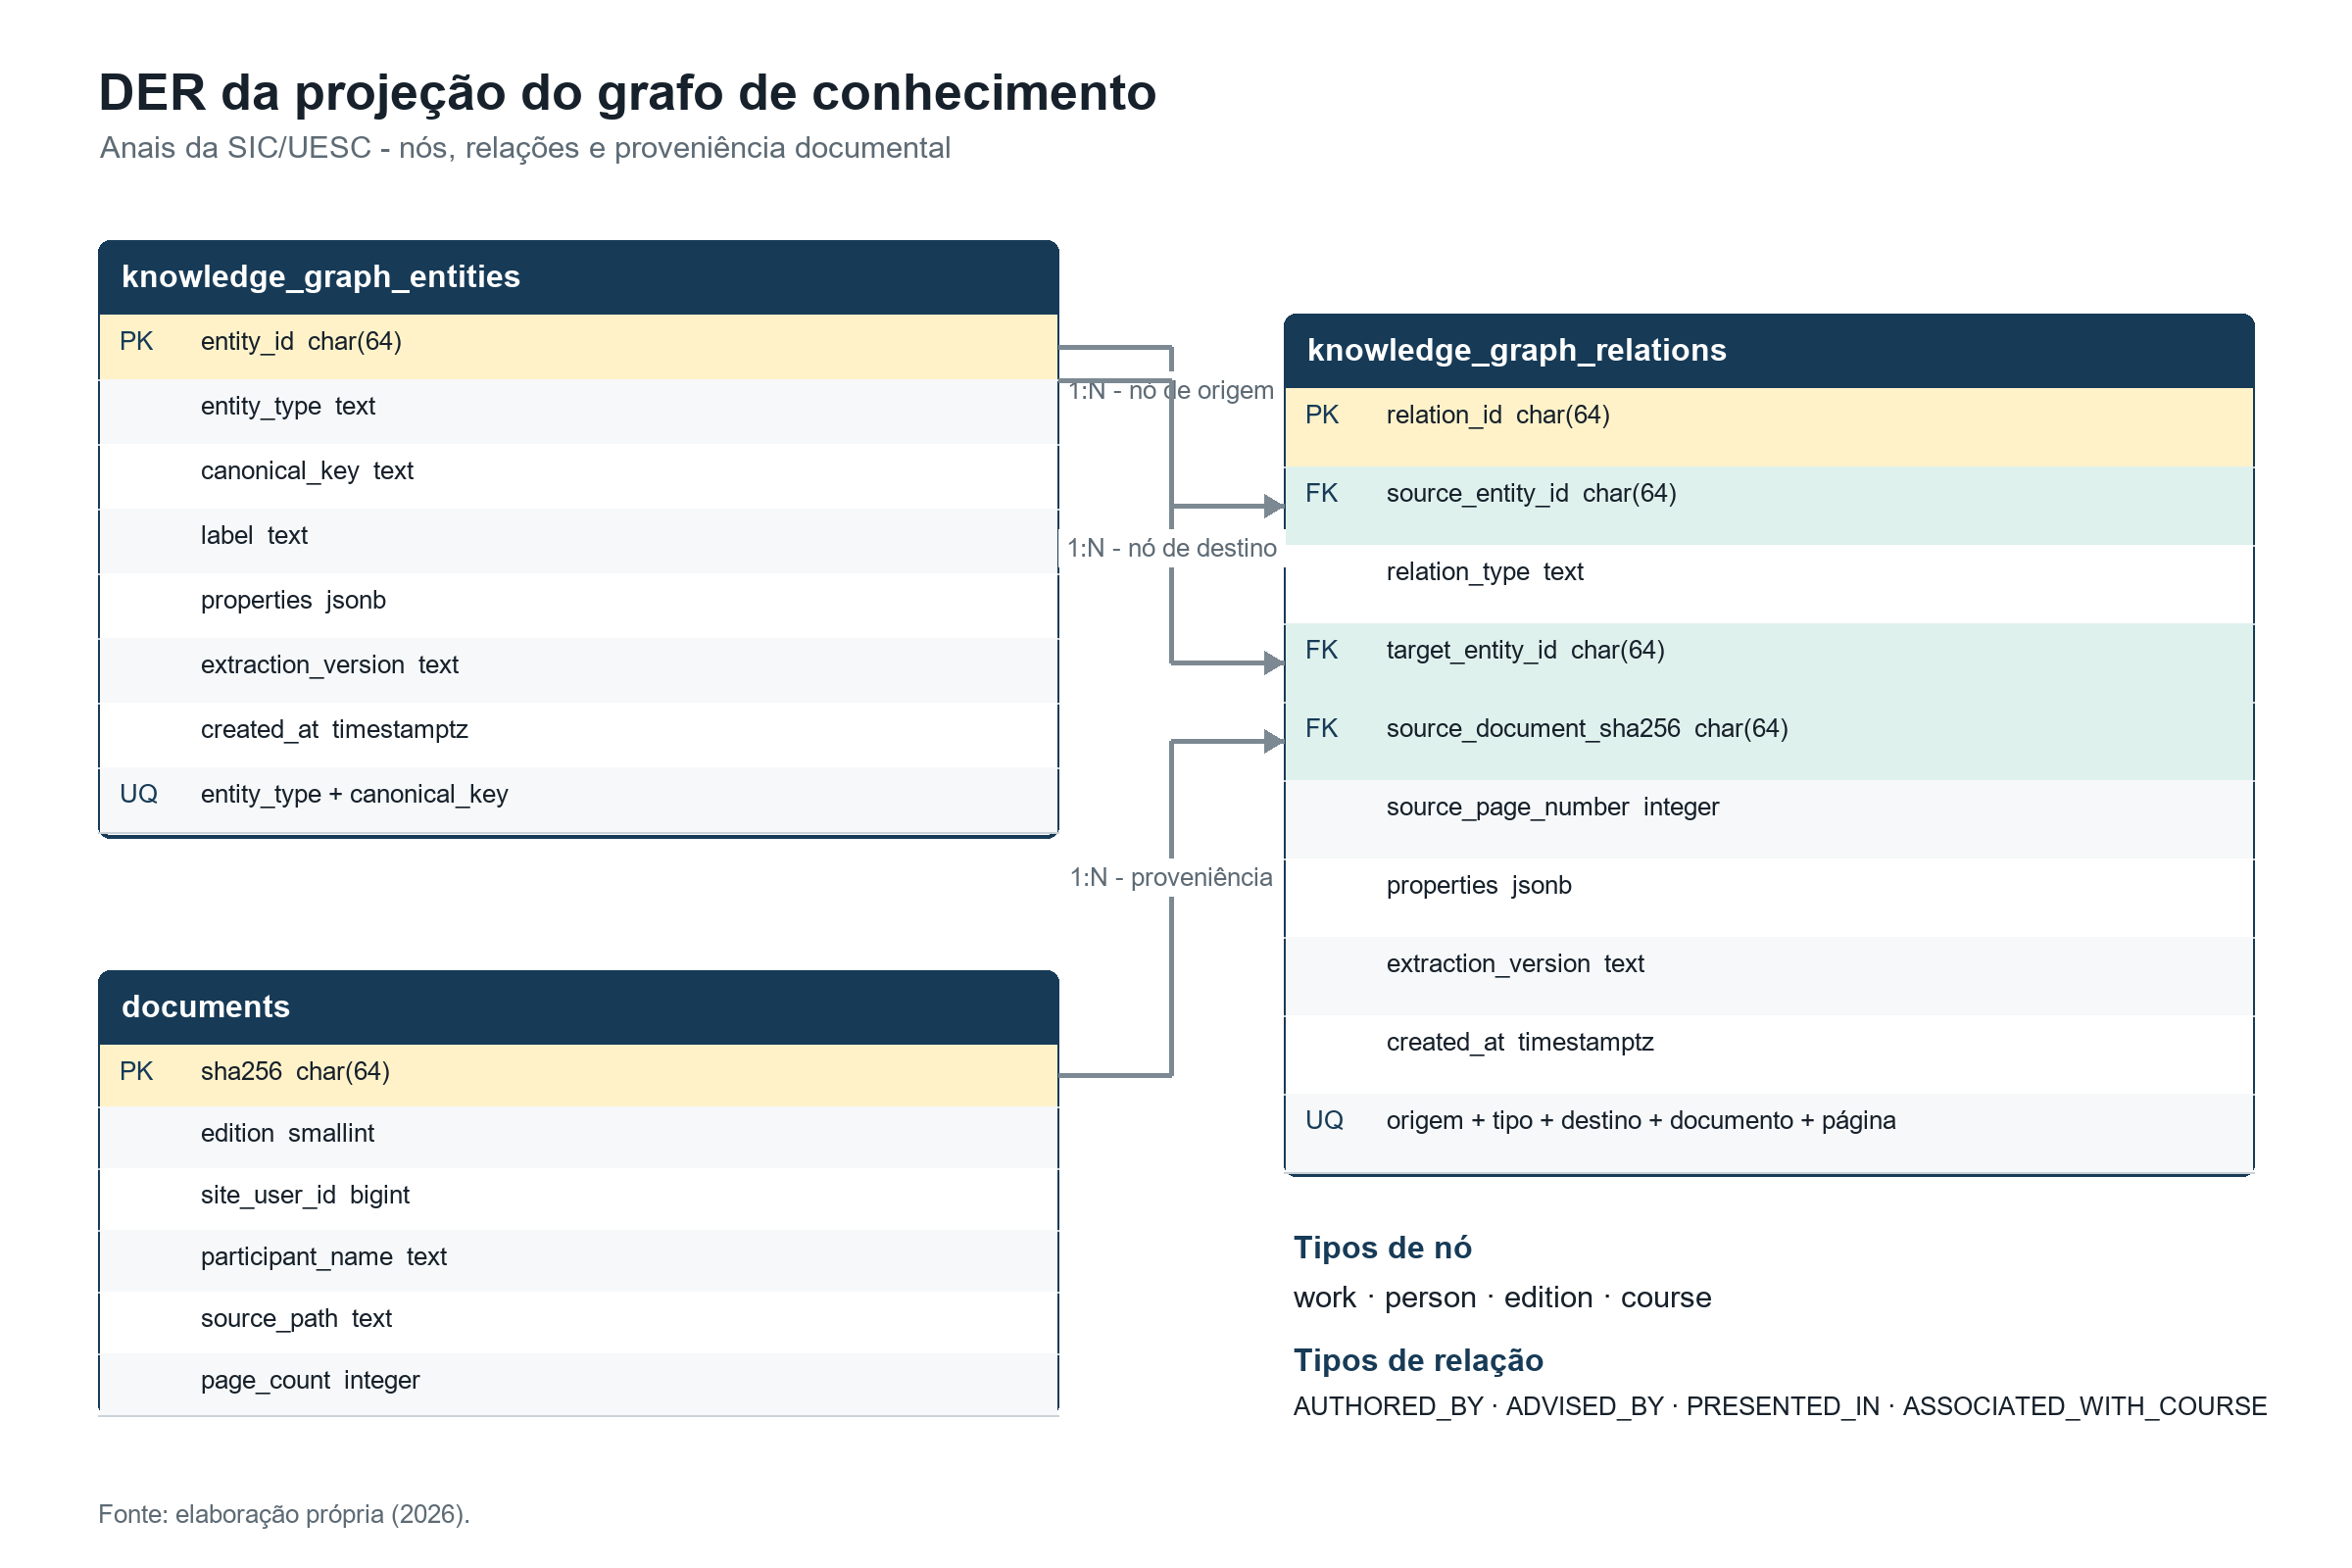
\includegraphics[width=\linewidth]{figuras/der_grafo_conhecimento.png}
\par\smallskip
{\setstretch{1}\footnotesize\textbf{Fonte:} Elaborada pelo autor (2026).\par}
\end{minipage}
\end{figure}

A Figura~\ref{fig:der-grafo-conhecimento} apresenta as tabelas implementadas. A tabela \path{knowledge_graph_entities} armazena os nós tipados, o rótulo de apresentação, a chave canônica, propriedades adicionais e a versão do extrator. A tabela \path{knowledge_graph_relations} armazena as arestas direcionadas, duas chaves estrangeiras para os nós de origem e destino e uma chave estrangeira para \texttt{documents}. A restrição de unicidade formada por origem, tipo, destino, documento e página impede a duplicação do mesmo vínculo proveniente da mesma evidência.

No DER, uma entidade pode participar de várias relações como origem ou destino, mas cada relação possui exatamente uma entidade de origem e uma de destino. Cada aresta também referencia um único documento, ao passo que um documento pode fundamentar várias relações. Essa cardinalidade permite representar, por exemplo, um trabalho ligado ao participante principal, ao orientador, à edição e ao curso, mantendo a proveniência de todos os vínculos. A chave estrangeira para \texttt{documents} integra o grafo à camada documental, e o SHA-256 do PDF funciona como identificador estável do trabalho em toda a arquitetura.

\subsection{Extração, normalização e carga}

O arquivo \path{src/rag_anais/graph_metadata.py} extrai os metadados da primeira página já armazenada na tabela \texttt{pages}. O procedimento localiza o participante principal a partir do metadado do portal, considera como título as linhas entre o código do trabalho e o bloco de autoria, lê o campo \texttt{CURSO:} e associa a numeração do bloco de autores à afiliação marcada como \textit{Orientador(a)}. Nenhuma relação de orientação é inferida pela LLM. Quando o marcador explícito não é encontrado, a aresta permanece ausente e o documento é registrado para revisão.

Nomes de pessoas e cursos são transformados em chaves canônicas por normalização de caixa, acentuação e espaços, enquanto o rótulo original é preservado para apresentação. O identificador de cada nó é um SHA-256 determinístico do tipo e da chave canônica. O identificador de cada aresta é calculado a partir da origem, do tipo, do destino e do documento de proveniência. Essa estratégia torna a carga idempotente: as mesmas entradas produzem os mesmos identificadores em novas execuções.

Antes da carga integral, quatro documentos de cada edição foram auditados, totalizando vinte registros. A amostra apresentou título, orientador e curso identificados em todos os casos. Em seguida, o programa \path{scripts/build_knowledge_graph.py} processou os 3.969 documentos em modo de prévia. A cobertura foi de 100,00\% para título, 99,90\% para orientador e 96,09\% para curso. Quatro documentos não apresentaram orientador identificável e 155 não apresentaram curso no formato reconhecido. Esses casos foram mantidos com relações parciais e preservados em \path{artifacts/knowledge_graph/knowledge_graph_warnings.csv}, sem preenchimento especulativo.

A gravação integral foi realizada em uma única transação com a versão \texttt{graph-metadata-v1}. A Tabela~\ref{tab:grafo-contagens} apresenta as quantidades produzidas.

\begin{table}[htbp]
\centering
\caption{Nós e relações da projeção do grafo de conhecimento}
\label{tab:grafo-contagens}
\renewcommand{\arraystretch}{1.18}
\small
\begin{tabular*}{\textwidth}{@{\extracolsep{\fill}}lrlr}
\toprule
\textbf{Tipo de nó} & \textbf{Quantidade} & \textbf{Tipo de relação} & \textbf{Quantidade} \\ \midrule
Trabalho & 3.969 & \texttt{AUTHORED\_BY} & 3.969 \\
Pessoa & 3.594 & \texttt{ADVISED\_BY} & 3.965 \\
Curso & 60 & \texttt{PRESENTED\_IN} & 3.969 \\
Edição & 5 & \texttt{ASSOCIATED\_WITH\_COURSE} & 3.814 \\ \bottomrule
\end{tabular*}
\fontetabela{Dados da carga do grafo de conhecimento (2026).}
\end{table}

\subsection{Roteamento e busca híbrida}

A projeção foi integrada à aplicação por meio do arquivo \path{src/rag_anais/graph_queries.py}. A função de roteamento normaliza a pergunta, identifica marcadores de agregação e extrai, quando presentes, nomes de autor, orientador, curso ou edição. A decisão é registrada com a versão \texttt{query-router-v1.2} e conduz a uma das três rotas a seguir:

\begin{enumerate}
    \item \textbf{estrutural}: utilizada para listas, contagens, rankings e relações explícitas. A resposta é montada diretamente a partir de consultas SQL parametrizadas sobre os nós e as arestas;
    \item \textbf{semântica}: utilizada quando a pergunta solicita temas, métodos, resultados ou outras evidências presentes no texto. Nesse caso, a recuperação vetorial continua sendo executada sobre o corpus integral;
    \item \textbf{híbrida}: utilizada quando a pergunta combina uma entidade estruturada com uma necessidade de informação textual, como ``quais trabalhos orientados por uma pessoa tratam de cacau?''.
\end{enumerate}

Na rota híbrida, o grafo atua primeiro como filtro. A entidade citada é localizada por sua chave canônica e suas arestas produzem a lista de SHA-256 dos documentos permitidos. Essa lista é entregue ao recuperador do arquivo \path{src/rag_anais/web_app.py}, que calcula o \textit{embedding} da pergunta com o modelo BGE-M3 e executa a busca por similaridade de cosseno no pgvector somente dentro desse subconjunto. Os fragmentos recuperados e ordenados formam o contexto enviado ao Llama~3 por meio do Ollama. Assim, o grafo define corretamente o universo documental, enquanto o recuperador semântico localiza as passagens relevantes e a LLM redige a resposta fundamentada.

O fluxo pode ser resumido como: pergunta $\rightarrow$ classificação da intenção $\rightarrow$ filtro relacional no grafo $\rightarrow$ recuperação vetorial restrita $\rightarrow$ montagem do contexto $\rightarrow$ geração da resposta. A separação é importante porque a LLM não deve estimar contagens nem inventar relações. Consultas quantitativas são calculadas pelo PostgreSQL; a LLM participa apenas quando há síntese de conteúdo textual. Cada execução é auditada em \texttt{query\_route\_runs}, que conserva rota, intenção, justificativa, versão do roteador, consulta executada, quantidade de documentos no escopo e duração. Isso permite reproduzir a decisão do sistema e comparar versões posteriores.

\subsection{Validação funcional do grafo e do roteamento}

O programa \path{scripts/validate_knowledge_graph.py} confirmou que os 3.969 documentos correspondem a 3.969 nós de trabalho. Cada trabalho possui uma relação de autoria principal e uma relação de edição. A verificação também confirmou a ausência de arestas órfãs e a correspondência entre as contagens por edição e o corpus auditado.

Em 21 de novembro de 2026, o roteador classificou corretamente as cinco perguntas da Tabela~\ref{tab:validacao-grafo-estrutural} como estruturais. O PostgreSQL produziu as respostas de forma determinística, com tempo médio de 11,86\,ms no ambiente local.

\begin{table}[!htbp]
\centering
\caption{Resultados da validação das consultas estruturais}
\label{tab:validacao-grafo-estrutural}
\small
\setlength{\tabcolsep}{5pt}
\renewcommand{\arraystretch}{1.12}
\begin{tabularx}{\textwidth}{>{\raggedright\arraybackslash}p{0.43\textwidth}>{\raggedright\arraybackslash}X}
\toprule
\textbf{Pergunta} & \textbf{Resultado} \\ \midrule
Quais foram os trabalhos apresentados por Breno Gonçalves Pirôpo? & \textit{Radar de Furto e Roubo de Veículos Automotores} (edição 4) e \textit{ConectCacau} (edição 5). \\
Quais trabalhos foram orientados por Gesil Sampaio Amarante Segundo? & 28 trabalhos nas edições 1 a 3, entre eles \textit{Preparação de conteúdos para o CDC-UESC}. \\
Quais trabalhos estão relacionados ao curso de Ciência da Computação? & 124 trabalhos, entre eles \textit{Gestão inteligente de água}. \\
Quantos trabalhos foram apresentados em cada edição da SIC/UESC? & Da edição 1 à 5, respectivamente: 680, 973, 733, 754 e 829. Total de 3.969 trabalhos. \\
Quais cursos apresentam mais trabalhos? & Enfermagem (288), Biomedicina (282) e Medicina Veterinária (276) lideram o ranking. \\ \bottomrule
\end{tabularx}
\fontetabela{Dados da validação funcional do grafo (2026).}
\end{table}

A verificação do roteamento, executada por \path{scripts/validate_graph_query_integration.py}, registrou 24 execuções sem erro. Na pergunta sobre cacau na edição 3, a rota híbrida limitou a busca vetorial aos 733 documentos da edição e retornou cinco resultados. Os resumos de carga e integridade e as respostas completas, com fontes e tempos individuais, constam em \path{artifacts/knowledge_graph/}, nos arquivos \path{knowledge_graph_build_summary.json}, \path{knowledge_graph_validation.json} e \path{experimento_grafo_5_perguntas.json}.

Os resultados descrevem a integridade do grafo e o funcionamento das rotas. A qualidade das respostas estruturais e híbridas permanece como objeto de avaliação humana futura. A consolidação por nome normalizado agrupou variações de grafia ou caixa em 343 chaves de pessoa. Homônimos podem exigir revisão dos vínculos no documento de origem.
